%version of 02-27-19

\chapter{SETS, BOOLEAN ALGEBRA, AND LOGIC}
\label{ch:sets-BA-logic}

\section{Sets}
\label{sec:sets}

\subsection{Fundamental Set-Related Concepts}
\label{sec:set-concepts}

Sets\index{Set} are probably the most basic object of mathematical
discourse.  Sets exist to have {\it elements},\index{Set!element} or
{\it members},\index{Set!member} the entities that {\em belong
  to}\index{Set!the belong-to relation} the set.  The notion of set is
surprisingly difficult to specify formally, so we just assume that
{\em the reader knows what a set is and recognizes that some sets are
  finite, while others are infinite}.  Speaking informally---a formal
treatment will follow in later chapters---here are a few illustrative
finite sets:
\begin{itemize}
\item
the set of words in this book

I do not know how big this set is, but I imagine that you as a reader
have a better idea than I as an author.
\item
the set of characters in any JAVA program

Note that while we are sure that this set is finite, we are not so
confident about the number of seconds the program will run!
\item
the set consisting of {\em you}

Paraphrasing the iconic television figure Mister Rogers, ``You are
unique.''  This set has just one element.

\item
the set of unicorns in New York City

I will not argue with you about this, but I believe that this is the
{\em empty set} $\emptyset$, which has zero members. 
\end{itemize}
Some familiar infinite sets are:
\begin{itemize}
\item
the set of {\em nonnegative integers}
\item
the set of {\em positive integers}
\item
the set of {\em all integers}
\item
the set of nonnegative {\em rational numbers}---which are quotients of
integers
\item
the set of nonnegative {\em real numbers}---which can be viewed
computationally as the set of numbers that admit infinite decimal
expansions,
\item
the set of nonnegative {\em complex numbers}---which can be viewed as
ordered pairs of real numbers,
\item
the set of {\em all} finite-length binary strings.

A {\it binary string}\index{Binary string} is a sequence of $0$s and
$1$s.  When discussing computer-related matters, one often calls each
$0$ and $1$ that occurs in a binary string a {\it bit}\index{Bit:
  binary digit} (for {\it binary digit}).  The term ``bit'' leads to
the term {\it bit string} as a synonym of {\it binary string}.
\end{itemize}
Despite this assumption, we begin the chapter by reviewing some basic
concepts concerning sets and operations thereon.

As noted early, sets were created to contain members/elements.  We
denote the fact that element $t$ {\it belongs to},\index{Set!the
  belongs to relation} or, {\it is an element of} set $T$ by the
notation $t \in T$\index{Set!membership: $\in$}.  A {\em
  subset}\index{Set!subset} of a set $T$ is a set $S$ each of whose
members belongs to $T$.  The subset relation occurs in two forms, The
{\em strong} form of the relation, denoted $S \subset
T$,\index{Set!strong subset relation} says that every element of $S$
is an element of $T$, but {\em not} conversely; i.e., $T$ contains
(one or more) elements that $S$ does not.  The {\em weak} form of the
relation, denoted $S \subseteq T$,\index{Set!weak subset relation}
is defined as follows:
\[
[S \subseteq T] \ \ \mbox{ means: } \ \
\Big[ \mbox{\em either } \ \ [S = T]
\ \ \mbox{\em or } \ \ [S \subset T] \Big].
\]

For any finite set $S$, we denote by $|S|$ the {\it cardinality}
\index{Set!cardinality}\index{cardinality!finite set} of $S$, which is
the number of elements in $S$.  Finite sets having three special
cardinalities are singled out with special names.  The limiting case
of finite sets is the unique {\em empty set}, which we denote by
$\emptyset$; thus, $\emptyset$ is characterized by the equation
$|\emptyset| = 0$.  (The empty set is often a limiting case of
set-defined entities.)  If $|S| = 1$, then we call $S$ a {\em
  singleton};\index{Set!singleton set} and if $|S| = 2$, then we call
$S$ a {\em doubleton}.\index{Set!doubleton}

It is often useful to have a convenient term and notation for {\em the
  set of all subsets of a set $S$}.  This bigger set---it contains
$2^{|S|}$ elements when $S$ is finite---is denoted by $\p(S)$ and is
called the {\em power set}\index{power set:set of all subsets} of
$S$.\footnote{The name ``power set'' arises from the relative
  cardinalities of $S$ and ${\cal P}(S)$ for finite $S$.}  Note
carefully the two set-relations that we are talking about here:

{\em A set $T$ that is a {\em subset} of set $S$ is an {\em element}
  of the set $\p(S)$.}

\noindent
You should satisfy yourself that the biggest and smallest elements of
${\cal P}(S)$ are, respectively, the set $S$ itself and the empty set
$\emptyset$.

\subsection{Operations on Sets}
\label{sec:set-operations}

Given two sets $S$ and $T$, we denote by:
\begin{itemize}
\item
$S \cap T$\index{$S \cap T$: set intersection} the {\it
  intersection}\index{Set!operations!intersection}
of $S$ and $T$: the set of elements that belong to {\em both} $S$ and
$T$.
\[ [s \in S \cap T] \ \ \mbox{ means } \ \ 
\Big[ [s \in S] \ \mbox{\bf and } \ [s \in T] \Big]
\]

\item
$S \cup T$\index{$S \cup T$: set union} the {\it
  union}\index{Set!operations!union}
of $S$ and $T$: the set of elements that belong to $S$, or to $T$, {\em
  or to both}.  (Because of the ``or both'' qualifier, this operation
is sometimes called {\em inclusive
  union}.)\index{Set!operations!inclusive union}
\[ [s \in S \cup T] \ \ \mbox{ means } \ \
\Big[ [s \in S] \ \mbox{\bf or } \ [s \in T]  \ \mbox{\bf or } \ [s
    \in S \cap T] \Big]
\]


\item
$S \setminus T$\index{$S \setminus T$: set difference} is the {\em
  (set) difference}\index{Set!operations!set difference} of $S$ and
  $T$: the set of elements that belong to $S$ but not to $T$.
\[ [s \in S \setminus T] \ \ \mbox{ means } \ \
\Big[ [s \in S] \ \mbox{\bf and } \ [s \not\in T] \Big]
\]
(Particularly in the United States, one often encounters the notation
 ``$S-T$''\index{$S - T$: set difference} instead of ``$S \setminus
 T$.'')
\end{itemize}

We illustrate the preceding operations with the sets $S = \{a,b,c\}$
and $T = \{c,d\}$.  For these sets:
\begin{eqnarray*}
S \cap T & = &  \{c\}, \\
S \cup T & = & \{a,b,c,d\}, \\
S \setminus T & = & \{a,b\}.
\end{eqnarray*}

In many set-related situations, the sets of interest will be subsets
of some fixed ``universal'' set $U$.\index{Set!universal set}
\begin{quote}
We use the term ``universal'' as in ``universe of discourse,'' not in
the self-referencing sense of a set that contains all other sets as
members, a construct (discussed by philosopher-logician Bertrand
Russell) \index{Russell, Bertrand} which leads to mind-bending paradoxes.
\end{quote}
Given a universal set $U$ and a {\em subset} $S \subseteq U$,
% (the notation meaning that every element of $S$---if there are any---is
%also an element of $U$)
we observe the set-inequalities
\[ \emptyset \ \subseteq \ S \ \subseteq \ U. \]
When studying a context within which there exists a universal set $U$
that contains all other sets of interest, we include within our
repertoire of set-related operations also the operation of {\it
  complementation}\index{Set!operations!complementation}
\begin{itemize}
\item
$\overline{S} \ \eqdef \ U \setminus S$,\index{$\overline{S}$: the
  complement of set $S$ relative to a universal set}
the {\em complement} of $S$ (relative to the universal set $U$).

For instance, the set of odd positive integers is the complement of
the set of even positive integers, relative to the set of all positive
integers.
\end{itemize}
We note a number of basic identities involving sets and operations on
them.
\begin{itemize}
\item
$S \setminus T \ = \ S \cap \overline{T}$,
\item
If $S \subseteq T$, then
  \begin{enumerate}
  \item
$S \setminus T \ = \ \emptyset$,
  \item
$S \cap T \ = \ S$,
  \item
$S \cup T \ = \ T$.
  \end{enumerate}
\end{itemize}
Note, in particular, that\footnote{``iff'' abbreviates the common
mathematical phrase, ``if and only if.''}
\[ [S = T] \ \mbox{  iff  } \ \ \Bigl[[S \subseteq T] \mbox{
    {\small\sf and} } [T \subseteq S]\Bigr] \ \mbox{  iff  }
\ \ \Bigl[ (S \setminus T) \cup (T \setminus S) = \emptyset\Bigr].
\]

The operations union, intersection, and complementation---and
operations formed from them, such as set difference---are usually
called the {\em Boolean (set) operations},
\index{Boolean set operations}\index{Set!operations!Boolean set operations}
named for the $19$th-century English mathematician George
Boole. \index{Boole, George} There are several important identities
involving the Boolean set operations.  Among the most frequently
invoked are the two ``laws'' attributed to the $19$th-century French
mathematician Auguste De Morgan:
\index{Set!operations!De Morgan's Laws}\index{De Morgan's Laws}
\begin{equation}
\label{e.de-morgan}
\mbox{For all sets $S$ and $T$: } \ \left\{
\begin{array}{lcl}
\overline{S \cup T} & = & \overline{S} \cap \overline{T}, \\
 \\
\overline{S \cap T} & = & \overline{S} \cup \overline{T}.
\end{array}
\right.
\end{equation}

\noindent {\em (Algebraic) Closure}.\index{(Algebraic) Closure}
%
We end this section with a set-theoretic definition that occurs in
many contexts.  Let $\cal C$ be any (finite or infinite) collection of
sets, and let $S$ and $T$ be two elements of $\cal C$.  (Note that
$\cal C$ is a set whose elements are sets.)  Think, e.g., of the
concrete example of set intersection.

We say that $\cal C$ is {\em closed} under intersection if whenever
sets $S$ and $T$ (which could be the same set) both belong to $\cal
C$, the set $S \cap T$ also belongs to $\cal C$.  By De Morgan's laws,
$\cal C$'s closure under union implies also its closure under
intersection.

\section{Binary Relations}
\label{s.relation}

\subsection{The Formal Notion of Binary Relation}
\label{s.relation-basic}

We begin our discussion of relations by adding a new (binary) set
operation to our earlier repertoire.  Given (finite or infinite) sets
$S$ and $T$ we denote by $S \times T$\index{$S \times T$} the {\it
  direct product} of $S$ and $T$,\index{direct product of sets} which
is the set of all {\it ordered pairs}\index{ordered pair of set
  elements} whose first coordinate contains an element of $S$ and
whose second coordinate contains an element of $T$.  For example, if
$S = \{a,b,c\}$ and $T = \{c,d\}$, then
\[ S \times T \ =  \{
\langle a,c \rangle,
\langle b,c \rangle,
\langle c,c \rangle,
\langle a,d \rangle,
\langle b,d \rangle,
\langle c,d \rangle\}
\]
The direct-product operation on sets affords us a simple, yet
powerful, formal notion of binary relation.

Given (finite or infinite) sets $S$ and $T$, a {\it relation $\rho$ on
  $S$ and $T$}\index{relation on sets} (in that order) is any subset
\[ \rho \ \subseteq \ S \times T. \]
When $S = T$, we often call $\rho$ a {\em binary relation on (the set)
  $S$}\index{binary relation on a set} (``{\em binary}'' because there
are {\em two} copies of set $S$ being related by $\rho$).

Relations are so common that we use them in every aspect of our lives
without even noticing them.  The relations ``equal to,'' ``less than,''
and ``greater than or equal to'' are simple examples of binary
relations on the integers.  These same three relations apply also to
other familiar number systems such as the rational and real numbers;
only ``equal,'' though, holds (in the natural way) for the complex
numbers.  Some subset of the three relations ``is a parent of,'' ``is
a child of,'' and ``is a sibling of'' probably are binary relations on
(the set of people constituting) your family.  To mention just one
relation with distinct sets $S$ and $T$, the relation ``$A$ is taking
course $X$'' is a relation on
\[ \left( \mbox{the set of all students} \right) \times
   \left( \mbox{the set of all courses} \right).
\]

\ignore{************
We shall see later (Section~\ref{s.pairing}) that there is a formal
sense in which binary relations are all we ever need consider: $3$-set
({\em ternary}) 
relations\index{ternary relation}\index{relation!ternary}---which are
subsets of $S_1 \times S_2 \times S_3$---and $4$-set ({\em
  quaternary}) 
relations\index{quaternary relation}\index{relation!quaternary}---which
are subsets of $S_1 \times S_2 \times S_3 \times S_4$---and so on (for
any finite ``arity''), can all be expressed as binary relations of
binary relations \ldots of binary relations.  As examples: For ternary
relations, we can replace any subset $R$ of $S_1 \times S_2 \times
S_3$ by the obvious corresponding subset $R'$ of $S_1 \times (S_2
\times S_3)$: for each element $\langle s_1, s_2, s_3 \rangle$ of $R$,
the corresponding element of $R'$ is $\langle s_1, \langle s_2, s_3
\rangle \rangle$.  Similarly, for quaternary relations, we can replace
any subset $R''$ of $S_1 \times S_2 \times S_3 \times S_4$ by the
obvious corresponding subset $R'''$ of $S_1 \times (S_2 \times (S_3
\times S_4))$: for each element $\langle s_1, s_2, s_3, s_4 \rangle$
of $R''$, the corresponding element of $R'''$ is $\langle s_1, \langle
s_2, \langle s_3, s_4 \rangle \rangle \rangle$.
\begin{quote}
You should convince yourself that we could achieve the desired
correspondence also by replacing $S_1 \times (S_2 \times S_3)$ with
$(S_1 \times S_2) \times S_3$ and by replacing $S_1 \times S_2 \times
S_3 \times S_4$ by either $((S_1 \times S_2) \times S_3) \times S_4$
or $(S_1 \times S_2) \times (S_3 \times S_4)$.
\end{quote}
************}

By convention, when dealing with a binary relation $\rho \ \subseteq
\ S \times T$, we often write ``$s \rho t$''\index{infix notation for
  a binary relation: $s \rho t$} in place of the more stilted notation
``$\langle s, t \rangle \in \rho$.''  For instance we (almost always)
write ``$5 < 7$'' in place of the strange-looking (but formally
correct) ``$\langle 5,7 \rangle \in \ <$.''

The following operation on relations occurs in many guises, in almost
all mathematical theories.  Let $\rho$ and $\rho'$ be binary relations
on a set $S$.  The {\it composition}
\index{composition! binary relations}
\index{composition of binary relations}
of $\rho$ and $\rho'$ (in that order) is the relation
\[ 
\rho'' \ \eqdef \ \Bigl\{ \langle s, t \rangle \in S \times S \ | \
(\exists t \in S) \Bigl[ [s \rho t] \mbox{ and } [t \rho' u] \Bigr] \Bigr\}.
\]
Note that we have used both of our notational conventions for
relations here.  We also encounter here, for the first time in the
text, but certainly not the last, a new notational convention: the
common ``shorthand'' compound symbol ``$\eqdef$'':
\index{$\eqdef$: ``equals, by definition''}
The sentence ``$X \eqdef Y$'' should be read ``$X$ {\em is (or, equals),
  by definition}, $Y$.''
\begin{quote}
The operation of composition of relations is quite important in the
study of ``relational'' databases.
\end{quote}

\noindent
It is important to be able to assert that elements $s, t \in S$ are
{\em not} $\rho$-related,\index{relation negation} i.e., $\langle s, t
\rangle \not\in S \times S$.  Several notations have been developed
for this purpose.\index{$\widetilde{\rho}$: the negation of relation $\rho$}
\begin{equation}
\label{eq:NOT-rho-notation}
\begin{array}{|c|c|c|c|}
\hline
\mbox{\bf Relation} & \mbox{\bf Notation} & \mbox{\bf Negation} &
\mbox{\bf Standard?} \\
\hline
\hline
\mbox{set membership} & \in & \not\in & \mbox{yes} \\
\hline
\mbox{equality}       & =   & \neq    & \mbox{yes} \\
\hline
\mbox{less than (strong)} & < & \not < \mbox{ or } \geq & \mbox{yes} \\
\hline
\mbox{less than (weak)} & \leq & \not\leq \mbox{ or } > & \mbox{yes} \\
\hline
\mbox{greater than (strong)} & > & \not > \mbox{ or } \leq & \mbox{yes} \\
\hline
\mbox{greater than (weak)} & \geq & \not\geq \mbox{ or } < & \mbox{yes} \\
\hline
\mbox{generic}  & \rho  & \sim\rho \mbox{ or } \widetilde{\rho} &
\mbox{no} \\
\hline
\end{array}
\end{equation}

There are several special classes of binary relations that are so
important that we must single them out immediately, in the following
subsections.


\subsection{Order Relations}
\label{sec:order-relation}

A binary relation $\rho$ on a set $S$ is a {\it partial order
  relation},\index{order relation}\index{order relation!
  partial}\index{partial order}\index{order} or, more briefly, is a
{\it partial order} if $\rho$ is transitive.\index{transitive
  relation} This means that, for all elements $s, t, u \in S$,
\begin{equation}
\label{eq:def-transitive}
\mbox{if } \ \ sRt \ \ \ \mbox{ and } \ \ tRu \ \ \ \mbox{ then }
\  \ sRu.
\end{equation}
The qualifier ``partial'' warns us that some pairs of elements of $S$
do not occur in relation $\rho$.  Number-related orders supply an easy
illustrative example.  Given any two distinct integers, $m$ and $n$,
one of them must be less than the other: either $m < n$, or $n < m$.
In contrast, if we consider {\it ordered pairs} of integers, then
there are pairs of pairs that are not related by the ``less than''
relation in any natural way.  For instance, even though we may agree
that, by a natural extension of the number-ordering relation ``less
than'', $\langle 4, 17 \rangle$ is ``less than'' $\langle 22, 19
\rangle$, we might well not agree on which of $\langle 4, 22 \rangle$
and $\langle 19, 17 \rangle$ is less than the other---or, indeed,
whether either is ``less than'' the other.

In many domains, order relations occur in two ``flavors'', {\em
  strong} and {\em weak}.\index{order!strong}\index{order!weak} For
many such relations $\rho$---consider, e.g., ``less than'' on the
integers---the weak version is denoted by underscoring the strong
one's symbol.  This will be our convention.  Just as $\leq$ denotes
the weak version of $<$, and $\geq$ denotes the weak version of $>$,
we shall denote the weak version of a generic order $\rho$ by
$\underline{\rho}$.\index{$\underline{\rho}$:the weak version of order
  relation $\rho$}.  Strong and weak versions of an order relation
$\rho$ (denoted, respectively, $\rho$ and $\underline{\rho}$) are
distinguished by their behavior under simultaneous membership.  For
illustration, instantiate the following template with $\rho$ being
``$<$'' and with $\rho$ being ``$>$'':

\smallskip

\begin{tabular}{lll}
For a strong order $\rho$: & &
{\bf if} $[s \ \rho \ t]$, {\bf then} $[t \ \widetilde{\rho} \ s]$ \\
For the weak version $\underline{\rho}$ of $\rho$: & &
{\bf if} $[s \ \underline{\rho} \ t]$ {\bf and} $[t \ \underline{\rho}
  \ s]$, {\bf then} $[s = t]$.
\end{tabular}

\subsection{Equivalence Relations}
\label{sec:equiv-relation}

A binary relation $R$ on a set $S$ is an {\it equivalence
  relation}\index{equivalence relation} if it enjoys the following
three properties:
\begin{enumerate}
\item
$R$ is {\em reflexive:} for all $s \in S$, we have $sRs$.
\item
$R$ is {\em symmetric:} for all $s, s' \in S$, we have $sRs'$ whenever
  $s'Rs$.
\item
$R$ is {\em transitive:} for all $s, s', s'' \in S$, whenever we have
  $sRs'$ and $s'Rs''$, we also have $sRs''$.
\end{enumerate}
Sample familiar  equivalence relations are:
\begin{itemize}
\item
The equality relation, $=$, on a set $S$ which relates each $s \in S$
with itself but with no other element of $S$.
\item
The relations $\equiv_{12}$ and $\equiv_{24}$ on integers,
where\footnote{As usual, $|x|$ is the {\em absolute value}, or, {\em
    magnitude} of the number $x$.  That is, if $x \geq 0$, then $|x| =
  x$; if $x < 0$, then $|x| = -x$.}
  \begin{enumerate}
  \item
$n_1 \equiv_{12} n_2$ if and only if $|n_1 - n_2|$ is divisible by
$12$.
  \item
$n_1 \equiv_{24} n_2$ if and only if $|n_1 - n_2|$ is divisible by
$24$.
  \end{enumerate}
We use relation $\equiv_{12}$ (without formally knowing it) whenever
we tell time using a $12$-hour clock and relation $\equiv_{24}$
whenever we tell time using a $24$-hour clock.
\end{itemize}

Closely related to the notion of an equivalence relation on a set $S$
is the notion of a {\it partition} of $S$.  A partition of $S$ is a
nonempty collection of subsets $S_1, S_2, \ldots$ of $S$ that are
\begin{enumerate}
\item
{\em mutually exclusive:}
for distinct indices $i$ and $j$, $S_i \cap S_j = \emptyset$;
\item
{\em collectively exhaustive:}
$S_1 \cup S_2 \cup \cdots = S$.
\end{enumerate}
We call each set $S_i$ a {\it block} of the partition.

One verifies the following Proposition easily.\index{partitions and
  equivalence relations} 

\begin{prop}
A partition of a set $S$ and an equivalence relation on $S$ are just
two ways of looking at the same concept.
\end{prop}

To verify this, we note the following.

\noindent {\small\sf Getting an equivalence relation from a partition}.
%
Given any partition $S_1, S_2, \ldots$ of a set $S$, define the
following relation $R$ on $S$:

\noindent
$sRs'$ if and only if $s$ and $s'$ belong to the same block of the
partition.

\noindent
{\em Relation $R$ is an equivalence relation on $S$.}
To wit, $R$ is reflexive, symmetric, and transitive because collective
exhaustiveness ensures that each $s \in S$ belongs to some block of
the partition, while mutual exclusivity ensures that it belongs to
only one block.

\noindent {\small\sf Getting a partition from an equivalence relation}.
%
To obtain the converse, focus on any equivalence relation $R$ on a set
$S$.  For each $s \in S$, denote by $[s]_R$ the set
\[ [s]_R \ \eqdef \ \{ s' \in S \ | \ sRs' \}; \]
we call $[s]_R$ {\it the equivalence class of $s$ under relation
$R$}.\index{equivalence class}\index{equivalence relation!class}

\noindent
{\em The equivalence classes under $R$ form a partition of $S$}.
To wit: $R$'s reflexivity ensures that the equivalence classes
collectively exhaust $S$; $R$'s symmetry and transitivity ensure that
equivalence classes are mutually disjoint.

The {\it index}\index{index (of an equivalence relation)} of the
equivalence relation $R$ is its number of classes---which can be
finite or infinite.

Let\footnote{Conforming to common usage, we typically use the symbol
  $\equiv$, possibly embellished by a subscript or superscript, to
  denote an equivalence relation.}~$\equiv_1$ and $\equiv_2$ be two
equivalence relations on a set $S$.  We say that the relation
$\equiv_1$ {\em is a refinement of} (or, {\em
  refines})\index{refinement of an equivalence relation} the relation
$\equiv_2$ just when each block of $\equiv_1$ is a subset of some
block of $\equiv_2$.  We leave to the reader the simple verification
of the following basic result.

\begin{theorem}
\label{thm:equality=finest-equiv}
The equality relation, $=$, on a set $S$ refines every equivalence
relation on $S$.  In this sense, it is the finest equivalence relation
on $S$.
\end{theorem}

\subsection{Functions}
\label{sec:function}

One learns early in school that a function from a set $A$ to a set $B$
is a rule that assigns a unique value from $B$ to every value from
$A$.  Simple examples illustrate that this notion of function is more
restrictive than necessary.  Think, e.g., of the operation {\em
  division} on integers.  We learn that division, like multiplication,
is a function that assigns a number to a given pair of numbers.  Yet
we are warned almost immediately not to ``divide by $0$'': The
quotient upon division by $0$ is ``undefined.''  So, division is not
quite a function as envisioned our initial definition of the notion.
Indeed, in contrast to an expression such as ``$4 \div 2$,'' which
should lead to the result $2$ in any programming
environment,\footnote{We are, of course, ignoring demons such as
  round-off error.}~expressions such as ``$4 \div 0$'' will lead to
wildly different results in different programming environments.  Since
``wildly different'' is anathema in any mathematical setting, we deal
with situations such as just described by broadening the definition of
``function'' in a way that behaves like our initial simple definition
under ``well-behaved'' circumstances and that extends the notion in an
intellectually consistent way under ``ill-behaved'' circumstances.
Let us begin to get formal.

A {\it (partial) function from set $S$ to set $T$} is a relation $F
\subseteq S \times T$ that is {\it single-valued;} i.e., for each $s
\in S$, there is {\em at most} one $t \in T$ such that $sFt$.  We
traditionally write ``$F: S \rightarrow T$'' as shorthand for the
assertion, ``$F$ is a function from the set $S$ to the set $T$''; we
also traditionally write ``$F(s) = t$'' for the more conservative
``$sFt$.''  (The single-valuedness of $F$ makes the nonconservative
notation safe.)  We often call the set $S$ the {\em source (set)},
\index{function!source set}
or, the {\it domain}
\index{function!domain}
%
of function $F$, and we call set $T$ the {\em target (set)}
\index{function!target set}
or, the {\it range}
\index{function!range}
%
of function $F$.  When there is always a (perforce, unique) $t \in T$
for each $s \in S$, then we call $F$ a {\em total} function.

\ignore{******* 
Note that our terminology is a bit unexpected: {\em Every total
  function is a partial function;} that is,
``partial''\index{function!partial} is the generic term, and ``total''
is a special case.
*********}

You may be surprised to encounter functions that are not total,
because most of the functions you deal with daily are {\em total}.
Our mathematical ancestors had to do some fancy footwork in order to
make your world so neat.  Their choreography took two complementary
forms.
\begin{enumerate}
\item
They expanded the target set $T$ on numerous occasions.  As just two
instances:
  \begin{itemize}
  \item
They appended both $0$ and the negative integers to the preexisting
positive integers\footnote{The great mathematician Leopold Kronecker
  said, ``God made the integers, all else is the work of man'';
  Kronecker was referring, of course, to the {\em positive}
  integers.}~in order to make subtraction a total function.

  \item
They appended the rationals to the preexisting integers in order to
make division (by nonzero numbers!)~a total function.
  \end{itemize}
The irrational algebraic numbers, the nonalgebraic real numbers, and
the nonreal complex numbers were similarly appended, in turn, to our
number system in order to make certain (more complicated) functions
total.

\item
They adapted the function.  In programming languages, in particular,
true undefinedness is anathema, so such languages typically have ways
of making functions total, via devices such as ``integer division''
(so that odd integers can be ``divided by $2$'') as well as various
ploys for accommodating ``division by $0$.''
\end{enumerate}
The ($20$th-century) inventors of {\em Computation Theory} insisted on
a theory of functions on nonnegative integers (or some transparent
encoding thereof).  The price for such ``pureness'' is that we must
allow functions to be undefined on some arguments.  Thus the theory
renders such functions as ``division by $2$'' and ``taking square
roots'' as being {\em nontotal}: both are defined only on subsets of
the positive integers (the even integers and the perfect squares,
respectively).

Three special classes of functions merit explicit mention.  For each,
we give both a down-to-earth name and a more scholarly Latinate one.

A function $F: S \rightarrow T$ is:
\begin{enumerate}
\item
{\it one-to-one} (or {\it injective}) if for each $t \in T$, there is
at most one $s \in S$ such that $F(s) = t$;

\medskip

{\em Example:}
\begin{itemize}
\item
 ``multiplication by $2$'' is injective:  If I give you an even
  integer $2n$, you can always respond by giving me $n$.
\item
``integer division by $2$'' is not injective---because performing the
  operation on arguments $2n$ and $2n+1$ yields the same answer
  (namely, $n$).
\end{itemize}

An injective function $F$ is called an {\it injection}.

\smallskip

Importantly, each injection $F$ has a {\it functional inverse},
\index{inverse of an injection}
%
which is commonly denoted $F^{-1}$.
\index{$F^{-1}$: functional inverse of injection $F$}
%
and which is defined as follows.  For each $t \in T$:
  \begin{itemize}
  \item
If there is an $s \in S$ such that $F(s) = t$, then
\[ F^{-1}(t) \ = \ s \]

  \item
If there is no $s \in S$ such that $F(s) = t$, then $F^{-1}(t)$ is not defined.
  \end{itemize}
Because $F$ is an {\em injection}, there is at most $s \in S$ such
that $F(s)= t$.  In other words, an element $t \in T$ can occur in the
range of $F$ only because of a single element $s \in S$ in the domain
of $F$.  This means that the preceding definition of $F^{-1}$ is a
valid definition (it is ``well-defined'') and that $F^{-1}$ is a
(partial) function $F^{-1}: T \rightarrow S$ whose domain is the range
of $F$.

\item
{\it onto} (or {\it surjective}) if for each $t \in T$, there is at
least one $s \in S$ such that $F(s) = t$;

\medskip

{\em Example:}
\begin{itemize}
\item
Two surjective functions on the nonnegative integers:
  \begin{itemize}
  \item
``subtraction of $1$'' is surjective, because ``addition of $1$'' is a
total function.
  \item
``taking the square root'' is surjective because the operation of
squaring is a total function.
  \end{itemize}
\item
Two functions on the nonnegative integers that are {\em not} surjective:
  \begin{itemize}
  \item
``addition of $1$'' is not surjective, because, e.g., $0$ is not ``$1$
greater'' than any nonnegative integer.
  \item
``squaring'' is not surjective, because, e.g., $2$ is not the
square of any integer.  (We prove this as
Proposition~\ref{thm:sqrt(2)}.) 
  \end{itemize}
\end{itemize}
A surjective function $F$ is called a {\it surjection}.

\item
{\it one-to-one, onto} (or {\it bijective}) if for each $t \in T$,
there is precisely one $s \in S$ such that $F(s) = t$.

\ignore{**********
{\em Example:} The (total) function $F: \{0,1\}^\star \rightarrow
\{0,1\}^\star$ defined by:
\[
(\forall w \in \{0,1\}^\star) \ F(w) \ = \
\mbox{(the reversal of $w$)}
\]
is a bijection.  The (total) function $F': \{0,1\}^\star \rightarrow
\N$ defined by
\[
(\forall w \in \{0,1\}^\star) \ F(w) \ = \
\mbox{(the integer that is represented by $w$ viewed as a numeral)}
\]
is {\em not} a bijection, due to the possibility of leading $0$'s.
\begin{quote}
A {\it numeral}\index{representation of integers!numeral}
is a sequence of digits that is the ``name'' of a number.  The
numerical value of a numeral $x$ depends on the {\it number 
base},\index{representation of integers!number base}
which is a positive integer $b >1$ that is used to create $x$.  Much
of our focus will be on {\em binary} numerals---which are binary
strings---for which the base is 
$b=2$.\index{representation of integers!base-$2$ representation}\index{representation of integers!binary representation}
For a general number base $b$, the integer denoted by the numeral
$\beta_n \beta_{n-1} \ldots \beta_1 \beta_0$, where each $\beta_i \in
\{0,1, \ldots, b-1\}$, is\index{representation of integers!base-$b$ representation}
\[ \sum_{i=0}^n \ \beta_i b^i. \]
We say that bit $\beta_i$ has {\em lower order}\index{representation of integers!low-order bit}
in the numeral than does $\beta_{i+1}$, because $\beta_i$ is
multiplied by $b^i$ in evaluating the numeral, whereas $\beta_{i+1}$
is multiplied by $b^{i+1}$.
\end{quote}
*********}

A bijective function $F$ is called a {\it bijection}.  When $F$ is a
bijection from $S$ onto $T$, we often write $F: S \leftrightarrow T$.
\end{enumerate}
There is a marvelous theorem that must be mentioned here, even though
it is beyond the scope of the book.\footnote{The theorem can be found
  in texts such as \cite{Birkhoff-MacLane53}.}
\index{The Schr\"{o}der-Bernstein Theorem}
%
The theorem says that, given sets $S$ and $T$: {\em if} there is an
injection $F_1$ that maps elements of $S$ one-to-one to elements of
$T$ {\em and} there is an injection $F_2$ that maps elements of $T$
one-to-one to elements of $S$, {\em then} there is a single bijection
$F$ such that
\begin{itemize}
\item
$F$ maps elements of $S$ one-to-one to elements of $T$;
\item
$F^{-1}$, the {\it functional inverse} of $F$,
\index{inverse of an injection}
maps elements of $T$ one-to-one to elements of $S$.
\end{itemize}

\begin{theorem}[The Schr\"{o}der-Bernstein Theorem]
For any sets $S$ and $T$, if there is an {\em injection} $F^{(S
  \rightarrow T)}: S \rightarrow T$ and an {\em injection} $F^{(T
  \rightarrow S)}: T \rightarrow S$, then there is a {\em bijection}
$F^{(S \leftrightarrow T)}: S \rightarrow T$.
\end{theorem}

\medskip

While the operation of {\it composition},
\index{composition!functions}
as introduced in Section~\ref{s.relation-basic}, is important for
general binary relations, it is a daily staple with relations that are
functions!  Let us be given two functions on a set $S$
\[
F: S \rightarrow S \ \ \ \ \mbox{ and } \ \ \ \ G: S \rightarrow S
\]
The composition of $F$ and $G$, {\em in that order}, is the function
\[ F \circ G: S \rightarrow S \]
defined as follows.
\begin{equation}
\label{eq:functions-composed}
\mbox{For each } \ s \in S \ \ \
F \circ G(s) \ = \ G(F(s)).
\end{equation}
The unexpected change in the orders of writing $F$ and $G$ on the two
sides of equation (\ref{eq:functions-composed}) results from the
existence of two historical schools that both contributed to the
formulation of this material.
\index{composition!functions!notation}
One school cleaved to the tradition of {\it abstract algebra}; they
wanted all expressions to be written with all operators---including
the composition operator $\circ$---in infix notation.  Another school,
which could be called {\it applicative algebraic}, wanted to view
functions as ``applying'' to their arguments.  Both notations have
significant advantages in certain contexts, so both have survived.  It
is a good idea for neophyte readers to be prepared to encounter both
notations---but they have to keep their eyes open regarding the
relative orders of $F$ and $G$.

\medskip

Before progressing with new material, it is worth taking a moment to
verify that the important operation of composition behaves the way one
would want and expect it to---by preserving the type of function being
composed.

\begin{prop}
\label{thm:fn-composition}
Let us be given functions $F: S \rightarrow S$ and $G: S \rightarrow
S$ on the set $S$, together with their composition $F \circ G$, as
defined in (\ref{eq:functions-composed}).

\noindent {\rm (a)}
$F \circ G$ is a function on $S$.

\noindent {\rm (b)}
If $F$ and $G$ are injections, then so also is $F \circ G$.

\noindent {\rm (c)}
If $F$ and $G$ are surjections, then so also is $F \circ G$.

\noindent {\rm (d)}
If $F$ and $G$ are bijections, then so also is $F \circ G$.
\end{prop}

\begin{proof}
We prove each of the four assertions by invoking the underlying
definitions.

\noindent (a)
%
Because $F$ and $G$ are functions on $S$: For each $s \in S$, there is
at most one $t_1 \in S$ such that $F(s) = t_1$ and at most one $t_2
\in S$ such that $G(s) = t_2$.  Hence, we identify three
possibilities.

\smallskip

\begin{tabular}{llll}
\hline
%1. &
{\bf if}
$F$ is defined at $s \in S$  & & & {\bf then} $F(s) \in S$ is unique \\
%  &
{\bf and if} $G$ is defined at $F(s) \in S$ & & & {\bf then} $G(F(s))
= F \circ G(s) \in S$ is unique \\
\hline
%2. &
{\bf if}
$F$ is not defined at $s \in S$ & & & {\bf then} $F \circ G$ is not
defined at $s \in S$ \\
\hline 
%3. & 
{\bf if}
$F$ is defined at $s \in S$ & & & {\bf then} $F(s) \in S$ is unique \\
%  &
{\bf and if} $G$ is not defined at $F(s) \in S$ & & & {\bf then}
$F \circ G$ not defined at $s \in S$ \\
\hline
\end{tabular}

\smallskip

\noindent
Hence, for each $s \in S$, there is at most one $t \in S$ such that $F
\circ G(s) = t$; in other words, $F \circ G$ is a function on $S$.

\medskip

\noindent (b)
%
Focus on any $s \in S$.  Because $F$ is an injection on $S$, there
exists at most one $t \in S$ such that $F(t) = s$.  Because $G$ is an
injection on $S$, there exists at most one $u \in S$ such that $G(u) =
t$.  Thus, there exists at most one $u \in S$ such that $F \circ G(u)
= s$.  Hence, $F \circ G(u)$ is an injection on $S$.

\medskip

\noindent (c)
%
Focus on any $s \in S$.  Because $F$ is a surjection on $S$, there
exists $t \in S$ such that $F(t) = s$.  Because $G$ is a surjection on
$S$, there exists $u \in S$ such that $G(u) = t$.  This means,
however, that $F \circ G(u) = s$.  Because $s \in S$ was arbitrary, it
follows that $F \circ G(u)$ is a surjection on $S$.

\medskip

\noindent (d)
%
If each of $F$ and $G$ is a bijection on $S$, then each is an
injection on $S$, and each is a surjection on $S$.  Then Part (b)
tells us that $F \circ G$ is an injection on $S$, and Part (c) tells
us that $F \circ G$ is a surjection on $S$.  Hence, $F \circ G$ is a
bijection on $S$.  \qed
\end{proof}


\section{Boolean Algebras}
\label{sec:Boolean-Algebra}
\index{Boolean Algebra}

A {\it Boolean algebra} is a mathematical system **HERE

\subsection{The Basics of Boolean Algebras}

\noindent {\it The Booean Operations}.
\index{Boolean Algebra!Operations}


\noindent{\it The Axioms of Boolean Algebras}.
\index{Boolean Algebra!axioms}

\noindent{The algebra of sets}.
\index{Boolean Algebra!the algebra of sets}

\subsection{The Algebra of Propositional Logic}
\label{sec:Propositional-logic}
\index{Propositional logic}\index{The Propositional Calculus}


\subsubsection{Logic via algebraic manipulation}


\noindent{The basic logical connectives}.
\index{Propositional logic!basic connectives}
%
The Boolean set-related operations we discussed in
Section~\ref{sec:set-operations} have important
analogues within the context of Propositional logic.
 {\em logical} analogues of these operations for logical
sentences and their logical {\em truth values},
\index{truth values}
%
{\sc true} and {\sc false}, often denoted $1$ and $0$, respectively:
\index{truth values!notations}
\begin{itemize}
\item
\underline{logical {\small\sf not} ($\sim$)}
\index{logical operation!{\sc not} ($\sim$)}
The operation {\small\sf not} is the logical analogue of the
set-theoretic operation of complementation.  Because always writing
``{\small\sf not}'' makes logical expressions long and cumbersome, we
usually use the prefix-operator $\sim$ to denote {\small\sf not};
i.e., we write \\
\hspace*{.35in}$\sim P$ \ \ rather than the more cumbersome
\ \ {\small\sf not} $P$ \\
to denote the logical complementation of proposition $P$.  Whichever
notation we use, the defining properties of logical complementation
are encapsulated in the following pair of equations
\[
[\sim \mbox{\sc true} = \mbox{\sc false}] \ \ \mbox{ and } \ \ [\sim
  \mbox{\sc false} = \mbox{\sc true}].
\]

\item
\underline{logical {\small\sf or} ($\vee$)}
\index{logical operation!{\small\sf or} ($\vee$)}
\index{logical operation!disjunction ($\vee$)}
\index{logical operation!logical sum ($\vee$)}
%
The operation {\small\sf or}---which is also called {\em disjunction}
or {\em logical sum}---is the logical analogue of the set-theoretic
operation of union.  For convenience and brevity, we usually use the
infix-operator $\vee$ to denote {\small\sf or} in expressions.
Whichever notation we use, the defining properties of logical
disjunction are encapsulated as follows.
\[
[[P \ \vee \ Q] =  \mbox{\sc true}] \ \ \mbox{ if, and only if, } \ \ 
[P = \mbox{\sc true}] \mbox{ or }
[Q = \mbox{\sc true}] \mbox{ or both}.
\]
Note that, as with union, logical {\small\sf or} is {\em inclusive:}
The assertion \\
\hspace*{.35in}$[P \vee Q]$ is \mbox{\sc true} \\
%
is true when {\em both} $P$ and $Q$ are true, as well as when only one
of them is.  Because such inclusivity does not always capture one's
intended meaning, another, {\em exclusive} version of disjunction also
exists, as we see next.

\item
\underline{logical {\small\sf xor} ($\oplus$)}
\index{logical operation!{\small\sf xor} ($\oplus$)}
\index{logical operation!exclusive or ($\oplus$)}
%
The operation {\em exclusive or}---which is also called {\small\sf
  xor}---is a version of disjunction that does not allow both
disjuncts to be true simultaneously.  For convenience and brevity, we
usually use the infix-operator $\oplus$ to denote {\small\sf xor} in
expressions.  Whichever notation we use, the defining properties of
exclusive or are encapsulated as follows. 
\[
[[P \ \oplus \ Q] =  \mbox{\sc true}] \ \ \mbox{ if, and only if, } \ \ 
[P = \mbox{\sc true}] \mbox{ or }
[Q = \mbox{\sc true}] \mbox{ {\em but not} both}.
\]
To emphasize the distinction between $\vee$ and $\oplus$: The
assertion \\
\hspace*{.35in}$[P \oplus Q]$ is \mbox{\sc true} \\
%
is {\em false} when {\em both} $P$ and $Q$ are true.

\item
\underline{logical {\small\sf and} ($\wedge$)}
\index{logical operation!{\small\sf and} ($\wedge$)}
\index{logical operation!conjunction ($\wedge$)}
\index{logical operation!logical product ($\wedge$)}
%
The operation {\small\sf and}---which is also called {\em conjunction}
or {\em logical product}---is the logical analogue of the
set-theoretic operation of intersection.  For convenience and brevity,
we usually use the infix-operator $\wedge$ to denote {\small\sf and}
in expressions.  Whichever notation we use, the defining properties of
logical conjunction are encapsulated as follows.
\[ [[P \ \wedge \ Q] = \mbox{\sc true}]  \ \ \mbox{ if, and only if,
  {\em both} } \ \ 
 [P = \mbox{\sc true}] \mbox{ and } [Q = \mbox{\sc true}]
\]

\item
\underline{logical implication ($\Rightarrow$)}
\index{logical operation!implies ($\Rightarrow$)}
\index{logical operation!implication ($\Rightarrow$)}
\index{logical operation!conditional ($\Rightarrow$)}
\index{logical operation!material implication ($\Rightarrow$)}
%
The logical operation of implication, which is often called {\it
  conditional} and which we usually denote in expressions via the
infix-operator $\Rightarrow$ differs from the other logical operations
we have discussed in a way that the reader must always keep in mind.
In contrast to {\small\sf not}, {\small\sf or}, and {\small\sf and},
whose formal versions pretty much coincide with their informal
versions, the formal version of implication, being formal, fixed, and
precise, carries connotations that we do not always associate with the
informal word ``implies.''  The formal version of implication is
defined as follows.
\[ [[P \ \Rightarrow \ Q] = \mbox{\sc true}]  \ \ \mbox{ if, and only
  if, } \ \
  [ [\sim P] = \mbox{\sc true}] \mbox{ (inclusive) or } [Q = \mbox{\sc true}]
\]
This definition means, in particular, that
  \begin{itemize}
  \item
If proposition $P$  is false, then it implies {\em every} proposition.
  \item
If proposition $Q$ is true, then it is implied by {\em every} proposition.
  \end{itemize}

\item
\underline{logical equivalence ($\equiv$)}
\index{logical operation!is equivalent to ($\equiv$)}
\index{logical operation!biconditional ($\equiv$)}
%
The final logical operation in our toolbox is variously called {\it
  equivalence,} as in: \\
\hspace*{.35in}Proposition $P$ is (logically) equivalent to
Proposition $Q$ \\
and {\it biconditional}.  We usually denote the operation in
expressions via the infix-operator $\equiv$.  The operation is defined
as follows.
\[ 
[[P \ \equiv \ Q] = \mbox{\sc true}]  \ \ \mbox{ if, and only if }
[[P \ \Rightarrow \ Q] = \mbox{\sc true}]  \ \ \mbox{ and } \ \
[[Q \ \Rightarrow \ P] = \mbox{\sc true}]
\]
\end{itemize}

We often use the term ``connective'' rather than ``operation'' to
refer to what we have here called the logical operations of the
Propositional Calclulus.  This is because one often feels that logical
propositions are static statements rather than active prescriptions
for computations.

\noindent {\it The (Boolean) algebra of logical operations}
\index{Propositional logic!logic as a Boolean algebra}
\index{the Boolean algebra of logical operations}
\index{Boolean algebra!the Propositional Calculus}

The operations of the Propositional Calclulus give rise to a Boolean
algebra that manipulates (logical) propositions in much the way that
the set-oriented Boolean algebra of
Section~\ref{sec:Boolean-Algebra-Sets} manipulates sets.


\subsubsection{Logic via Truth Tables}

\paragraph{\small\sf A. The logical connectives via truth tables}
\index{logical operations!a functional view}
%
If one is willing to view statements in the Propositional Calclulus as
prescriptions for computations, then one can encapsulate the
definitions of the basic logical connectives via functions that map
logical expressions int the truth values {\small\sf true}, or $1$, and
{\small\sf false}, or $0$.  The following tables reproduce the
definitions of Subsection~A within this computational framework.
\begin{equation}
\label{eq:defns-via-tables}
\begin{array}{|c||c|}
\hline
P & \sim P \\
\hline
\hline
0 & 1 \\
\hline
1 & 0 \\
\hline
\end{array}
\hspace*{.5in}
\begin{array}{|c|c||c||c||c||c||c|}
\hline
P & Q & P \vee Q  & P \oplus Q & P \wedge Q & P \Rightarrow Q & P \equiv Q  \\
\hline
\hline
0 & 0 & 0 & 0 & 0 & 1 & 1 \\
\hline
0 & 1 & 1 & 1 & 0 & 1 & 0 \\
\hline
1 & 0 & 1 & 1 & 0 & 0 & 0 \\
\hline
1 & 1 & 1 & 0 & 1 & 1 & 1 \\
\hline
\end{array}
\end{equation}

Note how the truth-value entries in the righthand truth table of
(\ref{eq:defns-via-tables}) reinforce the lessons of Subsection~A.
This awareness is especially essential with the implication-related
operations ($\Rightarrow$ and $\equiv$) that have informal
counterparts in ``real-life'' reasoning.  Think about whether your
intuition agrees with the formal specifications of these operations.

\smallskip

\paragraph {\small\sf D. Logic via truth values}
\index{Propositional logic!logic via truth values}

As demonstrated in Subsection~C, the Propositional Calculus is a
Boolean Algebra when one interprets the logical connectives of
Subsection~A as operations on logical expressions that evaluate to
either {\sc true} (or, $1$) or {\sc false} (or, $0$).  But, the
calculus forms a very special genre of Boolean Algebra, namely, a {\em
  free Boolean Algebra}.\index{Boolean algebra!{\em free} algebra}
\begin{quote}
The meaning of the qualifier {\it free} is easy to state but not so
easy to understand.  Here is a very informal try.

Any sort of algebra is defined as a set of objects accompanied by a
set of basic operations, wherein the operations obey certain
``self-evident'' \index{axioms as ``self-evident truths''}
axioms.\footnote{Indeed, that is what the word ``axiom'' means.}  In
rough, but evocative, terms, the algebra is {\em free} if its
operations do not relate to one another in any way that is not
mandated by the axioms.

An easy illustration of this decidedly {\em not easy} concept is the
following.  There is a (quite important) genre of algebra called a
{\it semi-group}.\index{semi-group} A semi-group $\s$ is specified via
a set (of objects) $S$, together with a binary operation on $S$, which
we denote $\oplus$.  For the (algebraic) structure $\s = \langle S,
\oplus \rangle$ to be a semi-group, it must obey the following two
axioms.
\begin{enumerate}
\item
$\s$ must be {\it closed} under operation $\oplus$; i.e., for all
  $s_1, s_2 \in S$, we must have
\[ (s_1 \oplus s_2) \in S. \]
\item
The operation $\oplus$ must obey the {\em associative law;}
\index{associative law}
i.e., for all $s_1, s_2, s_3 \in S$, we must have
\[ (s_1 \oplus s_2) \oplus s_3 \ = \ s_1 \oplus (s_2 \oplus s_3)
\]
\end{enumerate}

Now, it is easy to verify---we shall discuss this in
Chapter~\ref{ch:arithmetic}---that the (algebraic) structure formed by
the integers coupled with the operation of addition forms a semi-group
(which the notation of Chapter~\ref{ch:arithmetic} would denote
$\langle \Z, + \rangle$).  But this semi-group is {\em not}
free, because integer addition obeys laws beyond just closure and
associativity, namely:
\begin{enumerate}
\item
Addition of integers is {\em commutative}.
\item
Integer addition has an {\em identity}, namely $0$.
\item
Every integer $z \in \Z$ has an {\it additive inverse} (namely, $-z$).
\end{enumerate}

So, it really is meaningful that the Boolean Algebra built upon the
Porpositional calculus {\em is} free.
\end{quote}
For us, the impact of the ``freeness'' of the Propositional algebra,
{\it qua} Boolean Algebra, is manifest in the following
\index{meta-theorem}
{\em meta-theorem}\footnote{A {\it theorem} exposes some truth within
  the mathematical structure being discussed.  A {\it meta-theorem}
  exposes some truth about the way the discussion can proceed.}~which
is discussed and proved in \cite{Rosser53}.

\begin{theorem}
\label{thm:Prop-calc-isfree}
A propositional expression $E(P, Q, \ldots, R)$ is a theorem of
Propositional logic if, and only if, it to {\sc true} under all truth
assignments to the propositions $P, Q, \ldots, R$.
\end{theorem}

Proving Theorem~\ref{thm:Prop-calc-isfree} is beyond the scope of this
book, but we now present a few illustrative instantiations, annotated
to suggest their ``real-world'' messages.  Each example is accompanied
by a ``real-life'' interpretation and a verifying truth table.

\bigskip

\noindent
\underline{\small\sf The law of double negation} \\
\index{Propositional logic!Truth tables!the law of double negation}
\index{Truth tables!the law of double negation}
This is a formal analogue of the homely adage that ``a double negative
is a positive.''

\begin{prop}
\label{thm:double negation}
For any proposition $P$,
\[ P \ \ \equiv \ \ \sim [\sim P] \]
\end{prop}

\noindent {\it Proof via truth table.}
\begin{equation}
\label{eq:double-neg}
\begin{array}{|c|c||c|}
\hline
P & \sim P & \sim[\sim P] \\
\hline
\hline
0 & 1 & 0 \\
\hline
1 & 0 & 1 \\
\hline
\end{array}
\end{equation}
Note that columns 1 and 3 of truth table (\ref{eq:double-neg}) are
identical.  By Theorem~\ref{thm:Prop-calc-isfree}, this fact verifies
Proposition~\ref{thm:double negation}, the law of double negation.
\qed

\bigskip

\noindent 
\underline{\small\sf The law of contraposition} \\
\index{Propositional logic!Truth tables!the law of contraposition}
\index{Truth tables!the law of contraposition}
This is a very exciting example!  Let us immediately convert this to a
mathematical statement about the Boolean Algebra of Propositional
logic and then prove the statement.  We shall then contemplate the
implications of this law for {\em logic} rather than {\em
  mathematics}.\index{contraposition!inthe Boolean Algenra of propositions}

\begin{prop}
\label{thm:contraposition}
For any propositions $P$ and $Q$,
\[  \left[ [ P \Rightarrow Q ] \ \ \equiv \ \ [ \sim Q
    \Rightarrow \sim P ] \right]
\]
\end{prop}

\noindent {\it Proof via truth table.}
\begin{equation}
\label{eq:contraposition}
\begin{array}{|c|c|c|c||c||c|}
\hline
P & \sim P & Q & \sim Q & \underline{P \Rightarrow Q}
 & \underline{\sim Q \Rightarrow \sim P} \\
\hline
\hline
0 & 1 & 0 & 1 & 1 & 1 \\
\hline
0 & 1 & 1 & 0 & 1 & 1 \\
\hline
1 & 0 & 0 & 1 & 0 & 0 \\
\hline
1 & 0 & 1 & 0 & 1 & 1 \\
\hline
\end{array}
\end{equation}
Note that columns 5 and 6 of truth table (\ref{eq:contraposition}) are
identical.  By Theorem~\ref{thm:Prop-calc-isfree}, this fact verifies
Proposition~\ref{thm:contraposition}, the law of contraposition.
\qed

\smallskip

Now let us reconsider the whole concept of contraposition, including
this law, in the light of {\em logic and reasoning}.
\index{contraposition!in logic, reasoning}

 asserts that the assertion \\
\hspace*{.35in}
``Proposition $Q$ implies Proposition $Q$'' \\
is {\em logically equivalent} to the assertion \\
\hspace*{.35in}
``the negation of Proposition $Q$ implies the negation of Proposition
$P$''.  \\
Think about this!  In any system of reasoning in which a given
proposition is either {\small\sf true} or {\small\sf false} 





\bigskip

\noindent 
\underline{\it De Morgan's Laws}:\index{Propositional logic!Truth
  tables!verify De Morgan's Laws}\index{Truth tables!verify De Morgan's Laws}

\begin{prop}
\label{thm:De-Morgan}
For any propositions $P$ and $Q$:
\begin{itemize}
\item
$[ P \wedge Q ] \ \ \equiv \ \ \sim [ [\sim P] \vee [\sim Q]]$
\item
$[ P \vee Q ] \ \ \equiv \ \ \sim [ [\sim P] \wedge [\sim Q]]$
\end{itemize}
\end{prop}

\noindent {\it Proof via truth table.}
\begin{equation}
\label{eq:DeMorgan}
\begin{array}{|c|c|c|c||c|c|||c|c|}
\hline
P & \sim P & Q & \sim Q 
  & [ P \wedge Q ]
  & [\sim P] \vee [\sim Q]
  & [ P \vee Q ]
  & [\sim P] \wedge [\sim Q] \\
\hline
\hline
0 & 1 & 0 & 1
  & 0
  & 1
  & 0
  & 1 \\
\hline
0 & 1 & 1 & 0
  & 0
  & 1
  & 1
  & 1 \\
\hline
1 & 0 & 0 & 1
  & 0
  & 1
  & 1
  & 1 \\
\hline
1 & 0 & 1 & 0
  & 1
  & 0
  & 1
  & 0 \\
\hline
\end{array}
\end{equation}

Note that columns 5 and 6 of truth table (\ref{eq:DeMorgan}) are
mutually complementary, as are columns 7 and 8.  If we negate (or,
complement) the entries of columns 6 and 8, then we can invoke
Theorem~\ref{thm:Prop-calc-isfree} to verify
proposition~\ref{thm:De-Morgan}, which encapsulates De Morgan's laws
for Propositional logic.  \qed

\medskip

\noindent 
\underline{\small\sf The distributive laws for Propositional
  logic}\index{Propositional logic!Truth tables!the distributive
  laws}\index{Truth tables!the distributive laws for Propositional logic}


\noindent
In numerical arithmetic, multiplication distributes over addition, but
not conversely, so we have a single distributive law for arithmetic
(see Section~\ref{sec:Arithmetic-Laws}).  In contrast, each of logical
multiplication and logical addition distributes over the other, so we
have two distributive laws for Propositional logic.
\begin{itemize}
\item
$ P \vee [ Q \wedge R] \ \ \equiv \ \ [P \vee Q] \wedge R$
\item
$P \wedge [ Q \vee R] \ \ \equiv \ \ [P \wedge Q] \vee R$
\end{itemize}
{\small
\begin{equation}
\label{eq:distrib-law}
\begin{array}{|c|c|c||c|c|c|c|||c|c||c|c|}
\hline
P & Q & R
  & [P \vee Q]
  & [P \wedge Q]
  & [Q \wedge R] 
  & [Q \vee R] 
  & P \vee [ Q \wedge R]
  & [P \vee Q] \wedge [P \vee R]
  & P \wedge [ Q \vee R]
  & [P \wedge Q] \vee [P \wedge R] \\
\hline
\hline
0 & 0 & 0
  & 0
  & 0
  & 0
  & 0
  & 0
  & 0
  & 0
  & 0 \\ 
\hline
0 & 0 & 1
  & 0
  & 0
  & 0
  & 1
  & 0
  & 0
  & 0 
  & 0 \\
\hline
0 & 1 & 0
  & 1
  & 0
  & 0
  & 1
  & 0
  & 0
  & 0
  & 0 \\
\hline
0 & 1 & 1
  & 1
  & 0
  & 1
  & 1
  & 1
  & 1
  & 0
  & 0 \\
\hline
1 & 0 & 0
  & 1
  & 0
  & 0
  & 0
  & 1
  & 1
  & 0
  & 0 \\
\hline
1 & 0 & 1
  & 1
  & 0
  & 1
  & 0
  & 1
  & 1
  & 1
  & 1 \\
\hline
1 & 1 & 0
  & 1
  & 1
  & 0
  & 1
  & 1
  & 1
  & 1
  & 1 \\
\hline
1 & 1 & 1
  & 1
  & 1
  & 1
  & 1
  & 1
  & 1
  & 1
  & 1 \\
\hline
\end{array}
\end{equation}
}

Note that columns 8 and 9 of truth table (\ref{eq:distrib-law}) are
identical, as are columns 10 and 11.  By
Theorem~\ref{thm:Prop-calc-isfree} this fact verifies the distributive
laws for Propositional logic.

\subsection{Satisfiability problem}

Some basics

A \textit{literal} is a predicate composed of a single boolean variable $x$ or its negation.
A \textit{clause} is a particular predicate formed by disjunctions of literals, for instance $C = x \vee \bar{y} \vee z$.

The problem SAT (Satisfiability)  consists in deciding if there exists a truth assignment
that satisfies all the clauses of a given set of clauses. 
2SAT is the variant where the cardinality of the clauses is no more than $2$.
More formally, the problem is defined as follows:

Consider $n$ boolean variables and $m$ clauses $C_i$ composed of at most two literals on these variables. 

The question is to determine if there exists a truth assignment that satisfies 
the following boolean formula $C_1 \wedge C_2 \wedge ... \wedge C_m$.

SAT is well-known problem that plays a particular role in theoretical Computer Science since it was the first problem to be proved to be NP-complete. 
However, if we restrict the cardinality of the clauses to 2, 2SAT can be polynomially solvable.
This result can be proved elegantly by using graphs. Notice that the variant 3SAT (Clauses of cardinality $3)$ remains NP-complete. 
The idea is to transform the boolean formula $\Phi = C_1 \wedge C_2 \wedge ... \wedge C_m$ into a graph $G(\Phi)$
with $2n$ vertices where:

\begin{itemize}
\item
Each vertex corresponds to one variable in the two states $x$ and $\bar{x}$).
\item
Each clause $C_i = (a \vee b)$ is transformed into an arc between vertices $\bar{a}$ and $b$.

The meaning is to translate the fact that $b$ should be assigned to {\em true} in case if $a$ is {\em false}
(in other words, $\bar{a} \rightarrow b$). 
Controversally, there is an arc from $\bar{b}$ to $a$
if $b$ is {\em false}, $a$ should be {\em true}. 
\end{itemize}

In this graph, all the paths represent the valid logical implications. 

\begin{prop}
\label{prop:2SAT}
The boolean expression $\Phi = C_1 \wedge C_2 \wedge ... \wedge C_m$ is satisfiable iff
no strong component of $G(\Phi)$ contains both a vertex $x$ and its negation $\bar{x}$.
\end{prop}

The proof is a consequence of the two following elementary results.

\begin{prop}
\label{prop:2SATlemma1}
If $G(\Phi)$ contains a path from $x$ to $y$ then, it has a path from $\bar{y}$ to $\bar{x}$.
\end{prop}

The proof is easy by induction on the length of the shortest path from $x$ to $y$. 


\begin{prop}
\label{prop:2SATlemma2}
If $G(\Phi)$ contains a path from $x$ to $y$ then for every satisfying truth assignment $t$, $x(t)=1$ implies $y(t)=1$.
\end{prop}

\begin{proof}
Suppose that $\Phi$ is satisfied by a truth assignment $t$ where $x(t)=1$.
By contradiction, if along the path from $x$ to $\bar{x}$ , there exists an arc (say $\alpha,\beta$) such that $\alpha$ is {\em true} and $\beta$ is {\em false}.
As this arc belongs to $G(\Phi)$ it means that the clause ($\bar{\alpha},\beta$) is a clause of $\Phi$ 
whose assignment is ({\em false},{\em false}) and thus, the clause is not satisfied. 
\end{proof}
\medskip

Let us now prove the main result.

\begin{proof}
Suppose that $\Phi$ is satisfied by a truth assignment of $x$.
By first part of the proof is by contradiction, $\Phi$ is satisfiable by the truth assignment $t$.  
and there exists a strong component that contains both $x$ and $\bar{x}$.
From the previous result~\ref{prop:2SATlemma2}, $x(t)=1$ implies that $\bar{x}=1$, which is impossible. 

Let prove now that there is no strong component that contains bit a variable $x$ and its negation.
We construct as follows a truth assignment for $\Phi$:
Let order the strong component $S_i$ in the topologic order from $1$ to $k$,
that is, there is no arc from $S_j$ and $S_i$ if $i<j$.
Let mark all the non-assigned variables and start form the strong component which has the largest index.
We proceed backwards, if there is any variable in the current $S_i$ whose negation has been assigned, assign it to $0$
otherwise, assign it to $1$.
This way, all the clauses are satisfied.
Indeed assume by contradiction that there is a clause $\alpha \vee \beta$ which is not (this means that $\alpha = 0$
and then, $\bar{\alpha}$ has been assigned to $1$ before, in a strong component with a higher index.
The same stands for $\beta$ which is impossible since $\alpha \vee \beta$ corresponds to an arc $\bar{\alpha},\beta$.
\end{proof}


Let us develop two examples to illustrate this problem.
The first one $\Phi_1 = (\bar{x_{3}} \vee \bar{x_{1}}) \wedge (x_{1} \vee \bar{x_{2}}) \wedge (x_{2} \vee x_{3})$
is depicted in Fig.~\ref{2SATyes}). It leads to a positive truth assignment
while the second one $\Phi_2 = (\bar{x_{3}} \vee \bar{x_{1}}) \wedge (\bar{x_{1}} \vee {x_{3}}) \wedge (x_{2} \vee x_{3})$ (Fig.~\ref{2SATno}) is negative. 


\begin{figure}[h]
\begin{center}
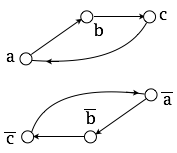
\includegraphics[width=0.3\textwidth]{FiguresGraph/2SATyes.png}
        \caption{There are two strong components that provides a truth assignment, for instance with $x_1=0, x_2=0, x_3=1$.}
\label{2SATyes}
\end{center}
\end{figure}

\begin{figure}[h]
\begin{center}
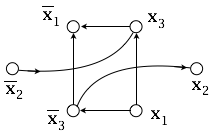
\includegraphics[width=0.3\textwidth]{FiguresGraph/2SATno.png}
        \caption{There exists a path from $x_1$ to $\bar{x_1}$, thus the formula can not be satisfied.}
\label{2SATno}
\end{center}
\end{figure}



\subsection{Connecting Mathematical Logic with Logical
  Reasoning}\index{Propositonal logic!connection with logical reasoning}
\label{sec:practical-logic}

\subsubsection{A formal notion of {\em implication}, and its
  implications}
\label{sec:implication}

In everyday discourse, we all employ an intuitive notion of {\it implication}.
\index{implication}
When we make the assertion \\
\hspace*{.35in}Proposition $A$ {\it implies} Proposition $B$ \\
what we usually have in mind is \\
\hspace*{.35in}If Proposition $A$ is true, then Proposition $B$ istrue. \\
But this, or any, homespun meaning of the word/concept ``implies''
raises many questions.
\begin{itemize}
\item
What if Proposition $A$ is {\em not} true?  Are there any inferences
we can draw?

\item
Is there any relation between the assertion \\
\hspace*{.35in}Proposition $A$ {\it implies} Proposition $B$ \\
and its {\it converse}\index{implication!converse}
assertion \\
\hspace*{.35in}Proposition $B$ {\it implies} Proposition $A$?

\item
If we know that Proposition $B$ is true, shouldn't it be ``implied by
every other proposition---perhaps even a {\em false} one?
\end{itemize}
This section is devoted to discussing the {\em formal} notion of
implication
\index{implication!formal notion}
\index{implication!formal notion!''pro and con''}
%
that was adopted by mathematical philosophers in the 19th century.
The {\em advantage} of having such a formal notion is that it will
answer all questions of the sort we have just posed.  The {\em
  disadvantage} of having such a formal notion is that the way in
which the notion answers some of our questions may be rather counter
to one's untutored intuition.
